\documentclass[11pt]{article}
\usepackage[spanish,es-tabla]{babel}
\usepackage{amsmath,amssymb}
\usepackage{graphicx}
\usepackage{geometry}
\usepackage{float}
\usepackage{setspace}
\usepackage{caption}
\captionsetup{labelfont=bf}
\usepackage{transparent}
\usepackage{fancyhdr}
\usepackage{xcolor} 
\usepackage{enumitem}
\usepackage[hidelinks]{hyperref}
\usepackage{tikz}
\geometry{margin=2.54cm}
\usepackage[style=apa]{biblatex}
\addbibresource{Referencias-Bibliograficas.bib}
\setstretch{1.5}
\pagestyle{fancy}
\usepackage{caption}
\usepackage{array}
\usepackage{titlesec}
\fancyhf{} 
\usepackage{booktabs}
\fancyhead[L]{
	\begin{minipage}{0.245\textwidth}
		
\includegraphics[width=4.2cm]{Logo-UIS/uis_horizontal.png}
	\end{minipage}
	\begin{minipage}{0.52\textwidth}
		\small
		Formación para la Investigación\\
		Escuela de Física, Facultad de Ciencias\\
		Universidad Industrial de Santander\\
		Construimos Futuro
	\end{minipage}
}

\fancyfoot[C]{\thepage}
\renewcommand{\headrulewidth}{0pt}
\renewcommand{\footrulewidth}{0pt}	

\definecolor{VerdeUIS}{RGB}{148, 193, 46}
\definecolor{VerdeUISTitulo}{RGB}{72, 74, 50}
\titleformat{\section}{\Large\bfseries\color{VerdeUISTitulo}}{\thesection}{1em}{}


\begin{document}
	
	\vspace*{0.1cm}
	\begin{center}
		{\Large \textbf{TÍTULO DEL PROYECTO DE INVESTIGACIÓN}}\\ %% el titulo debera ir en mayuscula todo indicando el I, ejemplo: I2. Determinación experimental del vector resultante de la suma de varias fuerzas concurrentes
		\vspace*{-0.4 cm}
		{\color{VerdeUIS}\rule{\textwidth}{1.4pt}} \\
		\textbf{Nombres y Apellidos del Autor 1.$^1$} Estudiante – Programa,\\
		\textbf{Nombres y Apellidos del Autor 2.$^2$} Estudiante – Programa,\\
		\textbf{Nombres y Apellidos del Autor 3.$^3$ }Estudiante – Programa,\\
		\textbf{Nombres y Apellidos del Autor 4.$^4$} Estudiante – Programa.\\
		\textbf{Nombres y Apellidos del profesor} Profesor@ – Laboratorio Física (I,II,III).\\ % aqui se debe quitar del () y dejar expresado Física I  y el Número al que corresponde la física.
		\textbf{Subgrupo X Grupo Y}.\\ %Subgrupo corresponde al A y el subrupo B, el Grupo sera el De la Combinación de letras
	\end{center}
	
	\vspace*{-0.9 cm}
	% INSTRUCCIÓN: Seleccionar una frase que para los autores sea significativa con relación al trabajo que realizaron e incluir el nombre del autor.
	\begin{flushright}
		\text{Frase Célebre: } \\
		``Si buscas resultados distintos, no hagas siempre lo mismo.'' \\  %esta frase se debe cambiar de acuerdo al laboratorio elaborado
		\textit{Albert Einstein}
	\end{flushright}
	
	\vspace*{-0.4 cm}
	
	Este documento es la plantilla para la elaboración del reporte de investigación de los proyectos de investigación de los laboratorios de física. El reporte de investigación se presenta en un formato de tipo artículo, con un máximo de 8 páginas de contenido, además de las referencias y la hoja de trabajo. Plantilla \LaTeX\ \textbf{elaborada} por el estudiante de\textbf{ Ingeniería de Sistemas} Diego Fernando Chamarraví Cáceres, Subido el Publico, a traves de \href{}{\textbf{GitHub}} \& \href{https://gitlab.com/MrChamarravi-Dev/plantilla-latex-informes-laboratorio-fisica-i-iii-universidad-industrial-de-santander.git}{\textbf{GitLab}} para la comunidad universitaria. (Este apartado se elimina, cada vez que se requiera hacer un nuevo informe).   
	
	\vspace*{-0.6 cm} %eliminar una vez se elimine el texto de arriba
	
	\section*{Resumen}
	\vspace*{-0.4 cm} 
	En el resumen se debe describir brevemente la experiencia y la principal conclusión del mismo, acorde con los objetivos del proyecto de investigación, con máximo de 300 palabras.  En el resumen se plantea el problema y los principales resultados obtenidos.  Es importante evitar la repetición de texto en el reporte de investigación, es decir, cada descripción debe aparecer en una sola parte de este documento.
	\vspace*{-0.6 cm} 
	\section*{Introducción}
	\vspace*{-0.4 cm} 
	En la introducción se amplía el planteamiento del problema, los objetivos, la pregunta de investigación o las hipótesis asociadas a la investigación, el estado del arte, una breve descripción del marco teórico, mencionando los principales conceptos con sus respectivas referencias.  Con respecto a los aspectos de forma, la redacción se debe realizar en \textbf{tercera persona}, singular o plural según corresponda.
	
	Como último párrafo de la introducción, se describen los componentes del documento.  Por ejemplo, para el caso de esta plantilla, se describiría que el documento está organizado en 6 componentes
	
	\newpage %pagina 2
	
	\vspace*{0.5cm} % ajustar de acuerdo a la vista previaque sea abajo de la parte superior
	
	fundamentales: Metodología y Equipo, Tratamiento de datos, Análisis de resultados, Conclusiones y Referencias, además de incluirse una breve descripción de cada uno de ellos.
	
	\vspace*{-0.72cm} % ajustar de acuerdo a la vista previaque sea abajo de la parte superior
	\section*{Metodología}
	\vspace*{-0.35cm} % ajustar de acuerdo a la vista previaque sea abajo de la parte superior
	La metodología responde a la pregunta: ¿cómo se hizo la investigación?  En esta parte del reporte de investigación se presenta una descripción detallada del procedimiento específico realizado en el desarrollo del proyecto de investigación mencionando los equipos utilizados. Se debe incluir un gráfico, dibujo o foto del montaje realizado en el desarrollo del experimento, titulado como se muestra al final de este documento.
	
	\vspace*{-0.72cm} % ajustar de acuerdo a la vista previaque sea abajo de la parte superior
	\section*{Tratamiento de Datos}
	\vspace*{-0.35cm} % ajustar de acuerdo a la vista previaque sea abajo de la parte superior
	En esta sección se incluye la tabla de datos, un cálculo tipo y una tabla donde se resuman los resultados con los cálculos realizados, además del cálculo del error, en caso que sea necesario.
	
	\vspace*{-0.72cm} % ajustar de acuerdo a la vista previaque sea abajo de la parte superior
	\section*{Análisis de Resultados}
	\vspace*{-0.35cm} % ajustar de acuerdo a la vista previaque sea abajo de la parte superior
	En esta sección se explican los resultados obtenidos y la comparación de dichos datos con los obtenidos por otros investigadores o los datos esperados  ( estos deben referenciarse), además, en lo posible, se deben incluir gráficos de análisis que muestren la relación entre las variables que hacen parte de la investigación.  Se recomienda primero comenzar con la identificación de las relaciones que los resultados indican.  Posteriormente, señalar los casos en los cuales no se encuentre correlación entre las variables.  De igual manera, se deben establecer los aspectos que no se pudieron resolver con el desarrollo de la experiencia, explicando las razones por las cuales se presentaron.  En este aspecto es importante no ocultar, alterar o forzar los datos, sino reconocer las limitaciones de los datos, de los instrumentos de medición y los posibles errores en el procedimiento de medición.
	
	Finalmente, se recomienda exponer las consecuencias teóricas de la investigación y las posibles aplicaciones de la misma.  El análisis de resultado guía el planteamiento de las conclusiones, pero no repite textualmente.
	
	Con respecto a las normas para la presentación de las gráficas deben ir centradas en el documento con su correspondiente título ubicado en la parte superior de la gráfica y en la parte inferior la fuente de la gráfica incluida. Un ejemplo se puede observar en la \textbf{figura 1}.
	
	Para el caso de las tablas, de igual manera se deben incluir centradas en línea con el texto, se debe seguir el formato que se muestra a continuación, que incluye título de la tabla y fuente de la misma. En caso de que los autores de la tabla o gráfica sean los mismos autores del documento,
	
	\newpage  %pagina 3
	\vspace*{0.5cm} % ajustar de acuerdo a la vista previaque sea abajo de la parte superior
	se debe identificar en la Fuente: Autor(es) del reporte de investigación, manteniendo los tipos de letra y demás aspectos gráficos proporcionados en el ejemplo.
	
	\vspace*{-0.01cm}
	
	\begin{figure}[H]
	\centering
	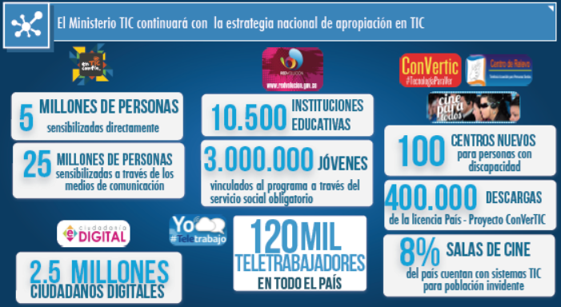
\includegraphics[width=0.98\textwidth]{Imagenes/figura1plantilla.png}
	\caption{Metas del Plan Vive Digital 2014-2018}
	\label{fig:1Imagen}
	\end{figure}
	
	\vspace*{-0.5cm}
	
	\noindent
	\textbf{Fuente:} Ministerio de Tecnologías de la Información y la Comunicación (2014) Plan Vive Digital 2014-2018. Recuperado de: http://www.vivedigital.gov.co/2014-2018/.
	
\begin{table}[H]
	\centering
	\footnotesize 
	\renewcommand{\arraystretch}{1.15} 
	
	\setlength{\arrayrulewidth}{0.2pt} 
	
	\begin{tabular}{|>{\raggedright\arraybackslash}p{5cm}|>{\centering\arraybackslash}p{3.5cm}|>{\centering\arraybackslash}p{3.5cm}|>{\centering\arraybackslash}p{3.5cm}|} 
		\hline
		& \textbf{Puntaje promedio} & \textbf{Margen de estimación} & \textbf{Intervalo de confianza} \\
		\hline
		Santander & 320 & $\pm 0,8$ & (319,2 -- 320,8)\\
		\hline
		Colombia & 301 & $\pm 0,2$ & (300,8 -- 301,2) \\
		\hline
		Establecimientos educativos oficiales urbanos de Santander & 315 & $\pm 1,1$ & (313,9 -- 316,1) \\
		\hline
		Establecimientos educativos oficiales urbanos de Colombia & 294 & $\pm 0,2$ & (293,8 -- 294,2) \\
		\hline
		Establecimientos educativos oficiales rurales de Santander & 296 & $\pm 1,8$ & (294,2 -- 297,8) \\
		\hline
		Establecimientos educativos oficiales rurales de Colombia & 273 & $\pm 0,3$ & (272,7 -- 273,3) \\
		\hline
		Establecimientos educativos no oficiales de Santander & 377 & $\pm 1,7$ & (375,3 -- 378,7) \\
		\hline
		Establecimientos educativos no oficiales de Colombia & 360 & $\pm 0,4$ & (359,6 -- 360,4) \\
		\hline
	\end{tabular}
	\caption{Comparación del puntaje promedio y el margen de estimación del departamento de Santander con el país y por tipos de establecimientos en lenguaje, tercer grado}
	\label{tab:mi_tabla}
\end{table}
	
\newpage %pagina 4
\vspace*{0.5cm} % ajustar de acuerdo a la vista previaque sea abajo de la parte superior
\textbf{Fuente:} ICFES (2014) Consulta de Resultados de Pruebas Saber Tercer grado en el área de Lenguaje en el departamento de Santander. Recuperado de: http://www2.icfesinteractivo.gov.co/ReportesSaber359/consultaReporteEntidadTerritorial.jspx 

\vspace*{-0.72cm} % ajustar de acuerdo a la vista previaque sea abajo de la parte superior
\section*{Referencias}
	\vspace*{-0.35cm} % ajustar de acuerdo a la vista previaque sea abajo de la parte superior
En esta sección se incluirían las referencias particulares utilizadas en la descripción de la experiencia. Todas las referencias deben ir adecuadamente escritas en normas APA, Colocarlas manual como el siguiente ejemplo:

% ============================
% EJEMPLO DE REFERENCIA (APA)
% ============================
%
% Apellido, A. A. (Año). \textit{Título del libro}. Editorial.
%

% Si la fuente fue consultada en línea:
%
% Serway, R. A. (1992). \textit{Physics for Scientists \& Engineers with Modern Physics}. Saunders College Publishing.
% Recuperado de: https://...

SERWAY, R. A. (1992). \textit{Physics for Scientists \& Engineers with Modern Physics / Raymond A. Serway}. Philadelphia: Saunders College Pub., 1992. Recuperado a partir de \url{http://search.ebscohost.com/login.aspx?direct=true&db=cat00066a&AN=BUIS.1-131923&lang=es&site=eds-live}

\vspace*{-0.70cm} % ajustar de acuerdo a la vista previaque sea abajo de la parte superior
\section*{Anexos}
	\vspace*{-0.35cm}
En esta sección deben ir las fotografías o imágenes escaneadas de las tablas de datos que registró en hoja de trabajo que usó durante la sesión práctica en el laboratorio, que incluye la fecha y firma de su profesor de Laboratorio.

\end{document}